\title{Impedance}
\author{
        Benjamin Shih \\
        Simple Explanations\\
}
\date{Last updated: \today}

\documentclass[12pt]{article}
\usepackage{graphicx}

\begin{document}
\maketitle

\section{Prerequisites}
\begin{itemize}
\item Complex Numbers
\item Frequency
\item Target Audience: 15
\end{itemize}


\section{An Explanation in Inductors and\newline Capacitors}

An impedance is a \textbf{complex number}:\\
\begin{center}
$z = s+j*w$
\end{center}

The real part, $s$, is called the \textbf{resistance}. It represents the opposition to current.

The complex part, $j*w$, is called the \textbf{reactance}. It represents the opposition to change in voltage due to capacitance (stores energy due to the electric field), or in current due to inductance (stores energy due to the magnetic field). \\
\begin{center}
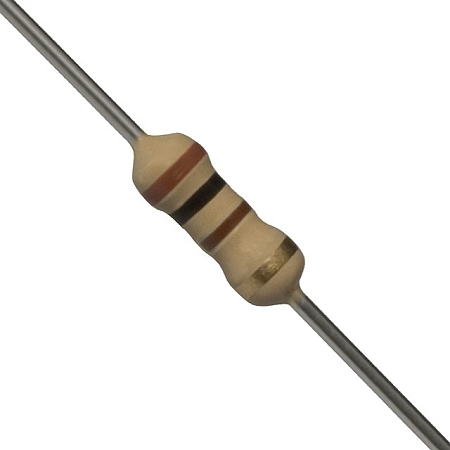
\includegraphics[height=50mm, width=50mm]{resistor.jpg}\\
A resistor has non-zero resistance, but has zero reactance. It takes the form\\

$z = a + j*0$\\
\end{center}

$w$ represents the frequency component of the impedance. In a capacitor, $z_C = \frac{1}{j*w*C}$. In an inductor, $z_L = j*w*L$.\\


\section{Simplifications at Extreme Frequencies}
For high and low frequencies, we can analyze the behavior of capacitors and inductors using limits:\\

\begin{center}
\begin{tabular}{|c|c|c|}
  \hline
  Impedance of \emph{col} at \emph{row} & Low Frequency & High Frequency\\
  \hline
  Capacitor & $\lim_{w \to 0} \frac{1}{j*w*C} = \infty$ & $\lim_{w \to \infty} \frac{1}{j*w*C} = 0$\\
  \hline
  Inductor & $\lim_{w \to 0} j*w*L = 0$ & $\lim_{w \to \infty} j*w*L = \infty$\\
  \hline
\end{tabular}
\end{center}

Theoretically, infinite impedance means that there is no connection between two points. On the other hand, zero impedance means that the two points are at the same potential. Translating from the above table to the context of electrical circuits:\\

\begin{center}
\begin{tabular}{|c|c|c|}
  \hline
   & Low Frequency & High Frequency\\
  \hline
  Capacitor & open circuit & short circuit\\
  \hline
  Inductor & short circuit & open circuit\\
  \hline
\end{tabular}
\end{center}

\newpage
\section{References}
\begin{itemize}
\item Carnegie Mellon Spring 2011 18220 Analog Devices and Semiconductors, Dr. David Greve
\item Carnegie Mellon Fall 2011 18320 Microelectronic Circuits, Dr. Jeyanandh Paramesh
\end{itemize}

\end{document}